 \definecolor{fondTI}{HTML}{869286}


\serie{Les nombres entiers}

\begin{exercice}[Un peu de vocabulaire]
Recopie et complète les phrases suivantes afin de les rendre exactes :
\begin{enumerate}
 \item Un \ldots \ldots \ldots est composé de chiffres ;
 \item 9 est un \ldots \ldots \ldots composé d'un seul \ldots \ldots \ldots ;
 \item Le chiffre des centaines du nombre 2\,568 est \ldots \ldots ;
 \item 3 est le chiffre des \ldots \ldots \ldots du nombre 783 ;
 \item \ldots \ldots est le chiffre des milliers du nombre 120\,452 ;
 \item Le chiffre des \ldots \ldots \ldots du nombre 43 est 4.
\end{enumerate}
\end{exercice}


\begin{exercice}[« Chiffre des » ou « nombre de »]
\begin{enumerate}
 \item Recopie et complète les phrases suivantes afin de les rendre exactes :
 \begin{itemize}
  \item $127 = 12 \cdot \ldots + 7$:
  
  127 possède donc \ldots \ldots dizaines ;
  \item $841\,123 = 841 \cdot \ldots + \ldots \ldots$ :
  
  841\,123 possède donc 841 \ldots \ldots ;
  \item $3\,816 = \ldots \cdot 100 + \ldots \ldots$ :
  
  \ldots \ldots possède donc \ldots \ldots .
  \end{itemize}
 \item Dans le nombre entier 15, quel est le nombre d'unités ? Le chiffre des unités ?
 \item Combien y a-t-il de centaines dans 4\,125 ?
 \item Quel est le chiffre des dizaines dans le nombre entier 498 ? Et le nombre de dizaines ?
 \item Dans 25 dizaines, quel est le nombre d'unités ?
 \end{enumerate}
\end{exercice}


\begin{exercice}
Donne l'écriture en chiffres des nombres entiers suivants :
\begin{enumerate}
 \item $(9 \cdot 10) + 5$ ;
 \item $(7 \cdot 1\,000) + (5 \cdot 100) + (2 \cdot 10) + 8$ ;
 \item $(1 \cdot 10\,000) + (1 \cdot 100) + 1$ ;
 \item  $(3 \cdot 100\,000) + (7 \cdot 10\,000) + (4 \cdot 10) + 9$ ;
 \item  $(3 \cdot 100\,000) + (4 \cdot 100) + (7 \cdot 1\,000) + 9$.
 \end{enumerate}
\end{exercice}


\begin{exercice}
Écris en chiffres les nombres suivants :
\begin{enumerate}
 \item Sept mille huit cent douze ;
 \item Soixante-trois mille neuf cent cinquante ;
 \item Huit millions trois ;
 \item Septante-quatre milliards cent quatre ;
 \item Cent trente-six millions huit cent nonante-trois mille sept cent cinq.
 \end{enumerate}
\end{exercice}

\begin{exercice}
Classe les nombres suivants dans l'ordre décroissant (du plus grand au plus petit) :
\begin{colitemize}{2}
 \item 23\,100 ;
 \item Cent vingt-trois mille ;
 \item 1\,320 ;
 \item Mille cent vingt-trois.
 \end{colitemize}
\end{exercice}

%%%%%%%%%%%%%%%%%%%%%%%%%%%%%%%%%%%%%%%%%%%%%%%%%%%%%%%%%%%%%%%%%%%%%%%%%%%

\serie{Les nombres décimaux}

\begin{exercice}[Combien de \ldots dans \ldots ?]
\begin{enumerate}
 \item Combien de millièmes y a-t-il dans une unité ?
Traduis cela par une égalité mathématique.
 \item Combien de centièmes y a-t-il dans une unité ? Traduis cela par une égalité mathématique.
 \item Combien de centièmes y a-t-il dans un dixième d'unité ? Traduis cela par une égalité mathématique.
 \end{enumerate}
\end{exercice}


\begin{exercice}
Complète les égalités :
\begin{enumerate}
 \item 4 unités 6 dixièmes = \ldots \ldots dixièmes ;
 \item  \ldots \ldots  unité \ldots \ldots centièmes = 123 centièmes ;
 \item 12 unités 37 millièmes = \ldots \ldots millièmes.
 \end{enumerate}
\end{exercice}


\begin{exercice}
Donne une écriture décimale des nombres suivants :
\begin{enumerate}
 \item Sept unités et huit dixièmes \dotfill ;
 \item Cent unités, huit dixièmes et un centième
 
 \dotfill ;
 \item Deux unités et trois centièmes
 
 \dotfill ;
 \item Treize centaines \dotfill ;
 \item Trente-six milliers et huit millièmes
 
 \dotfill ;
 \item Cinq unités et quinze millièmes \dotfill.
 \end{enumerate}
\end{exercice}


\begin{exercice}[Sur une demi-droite graduée]
Donne les abscisses des points $A$, $B$ et $C$, sous la forme d'un nombre décimal.
\begin{center} 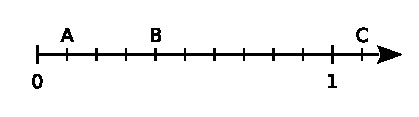
\includegraphics[width=7cm]{axe0AB1C} \end{center}
\end{exercice}

\begin{exercice}[Dans un sens]
Donne l'écriture décimale :
\begin{enumerate} 
 \item 75 milliers \dotfill ; 

 \item 5 centièmes \dotfill ; 

 \item 13 dizaines \dotfill ; 

 \item 9 dixièmes \dotfill ; 

 \item 35 centaines \dotfill ;

 \item 956 millièmes \dotfill. 

 \end{enumerate}
\end{exercice}


\begin{exercice}[Vocabulaire des nombres décimaux]
\begin{enumerate}
 \item Quel est le chiffre des millièmes de 24,738 ?
 
 \dotfill ;
 \item Quel est le nombre de millièmes de 24,738 ?
 
 \dotfill ;
 \item Que représente le chiffre 3 dans 7\,859,342 ?
 
 \dotfill ;
 \item Quel est le nombre de centièmes de 17,78 ?
 
 \dotfill ;
 \item Quel est le chiffre des centièmes de 71,865 ?
 
 \dotfill ;
 \item Donne la partie entière du nombre 83,712 :
 
 \dotfill ;
 \item Donne la partie décimale du nombre 54,91 :
 
 \dotfill.
 \end{enumerate}
\end{exercice}


\begin{exercice}
Trouve un nombre à cinq chiffres ayant 7 pour chiffre des dizaines, 9 pour chiffre des centièmes, 0 pour chiffre des unités, 3 pour chiffre des millièmes et comme autre chiffre 1.
\end{exercice}


\begin{exercice}[Devinette]
Trouve le nombre ayant les caractéristiques suivantes :
\begin{itemize}
 \item il n'a que deux chiffres après la virgule ;
 \item il a la même partie entière que 1 890,893 ;
 \item son chiffre des centièmes est le même que celui de 320,815 ;
 \item son chiffre des dixièmes est égal à la moitié de celui de 798,635.
 \end{itemize}
\end{exercice}


\begin{exercice}[Zéros inutiles]
Écris, lorsque cela est possible, les nombres suivants avec moins de chiffres.
\begin{enumerate} 
 \item 17,200 \dotfill ; 
 
 \item 123,201 \dotfill ; 
  
 \item 36,700\,10 \dotfill ; 
 
 \item 0\,021,125 \dotfill ; 
 
 \item 0,123\,0 \dotfill ; 
 
 \item 023,201\,20 \dotfill ; 
 
 \item 30,000 \dotfill ; 
 
 \item 0\,050,12 \dotfill ; 
 
 \item 1\,205\,500,0 \dotfill. 
  
 \end{enumerate}
\end{exercice}


\begin{exercice}[Décomposition]
Donne une écriture décimale qui correspond à chacune des décompositions suivantes :
\begin{enumerate}
 \item $(3 \cdot 10) + (4 \cdot 1) + (4 \cdot 0,1) + (7 \cdot 0,01)$
 \item $(8 \cdot 100) + (5 \cdot 1) + (9 \cdot 0,1) + (6 \cdot 0,01)$
 \item $(5 \cdot 1) + (4 \cdot 0,01) + (3 \cdot 0,001)$
 \item $(7 \cdot 100) + (9 \cdot 1) + (8 \cdot 0,1) + (6 \cdot 0,001)$
 \end{enumerate}
\end{exercice}


\begin{exercice}[Décomposition (bis)]
Décompose chacun de ces nombres de la même façon qu'à l'exercice précédent :
\begin{enumerate} 
 \item 9,6 \dotfill ; 
 
 \item 84,258 \dotfill ; 
 
 \item 7,102 \dotfill ;
 
 \item 123,015 \dotfill ; 
 
 \item 0,008\,3 \dotfill ; 
 
 \item 1\,002,200\,4 \dotfill.
 
 \end{enumerate}
\end{exercice}


\begin{exercice}
Sur la demi-droite graduée ci-dessous, place les points $O(0)$, $A(1)$, $B(2)$, $C(0,5)$, $D(1,6)$, $E(0,1 + 0,05)$, $F(0,2)$, $G(1 + 0,05)$ et $H(1,45)$ :
\begin{center} 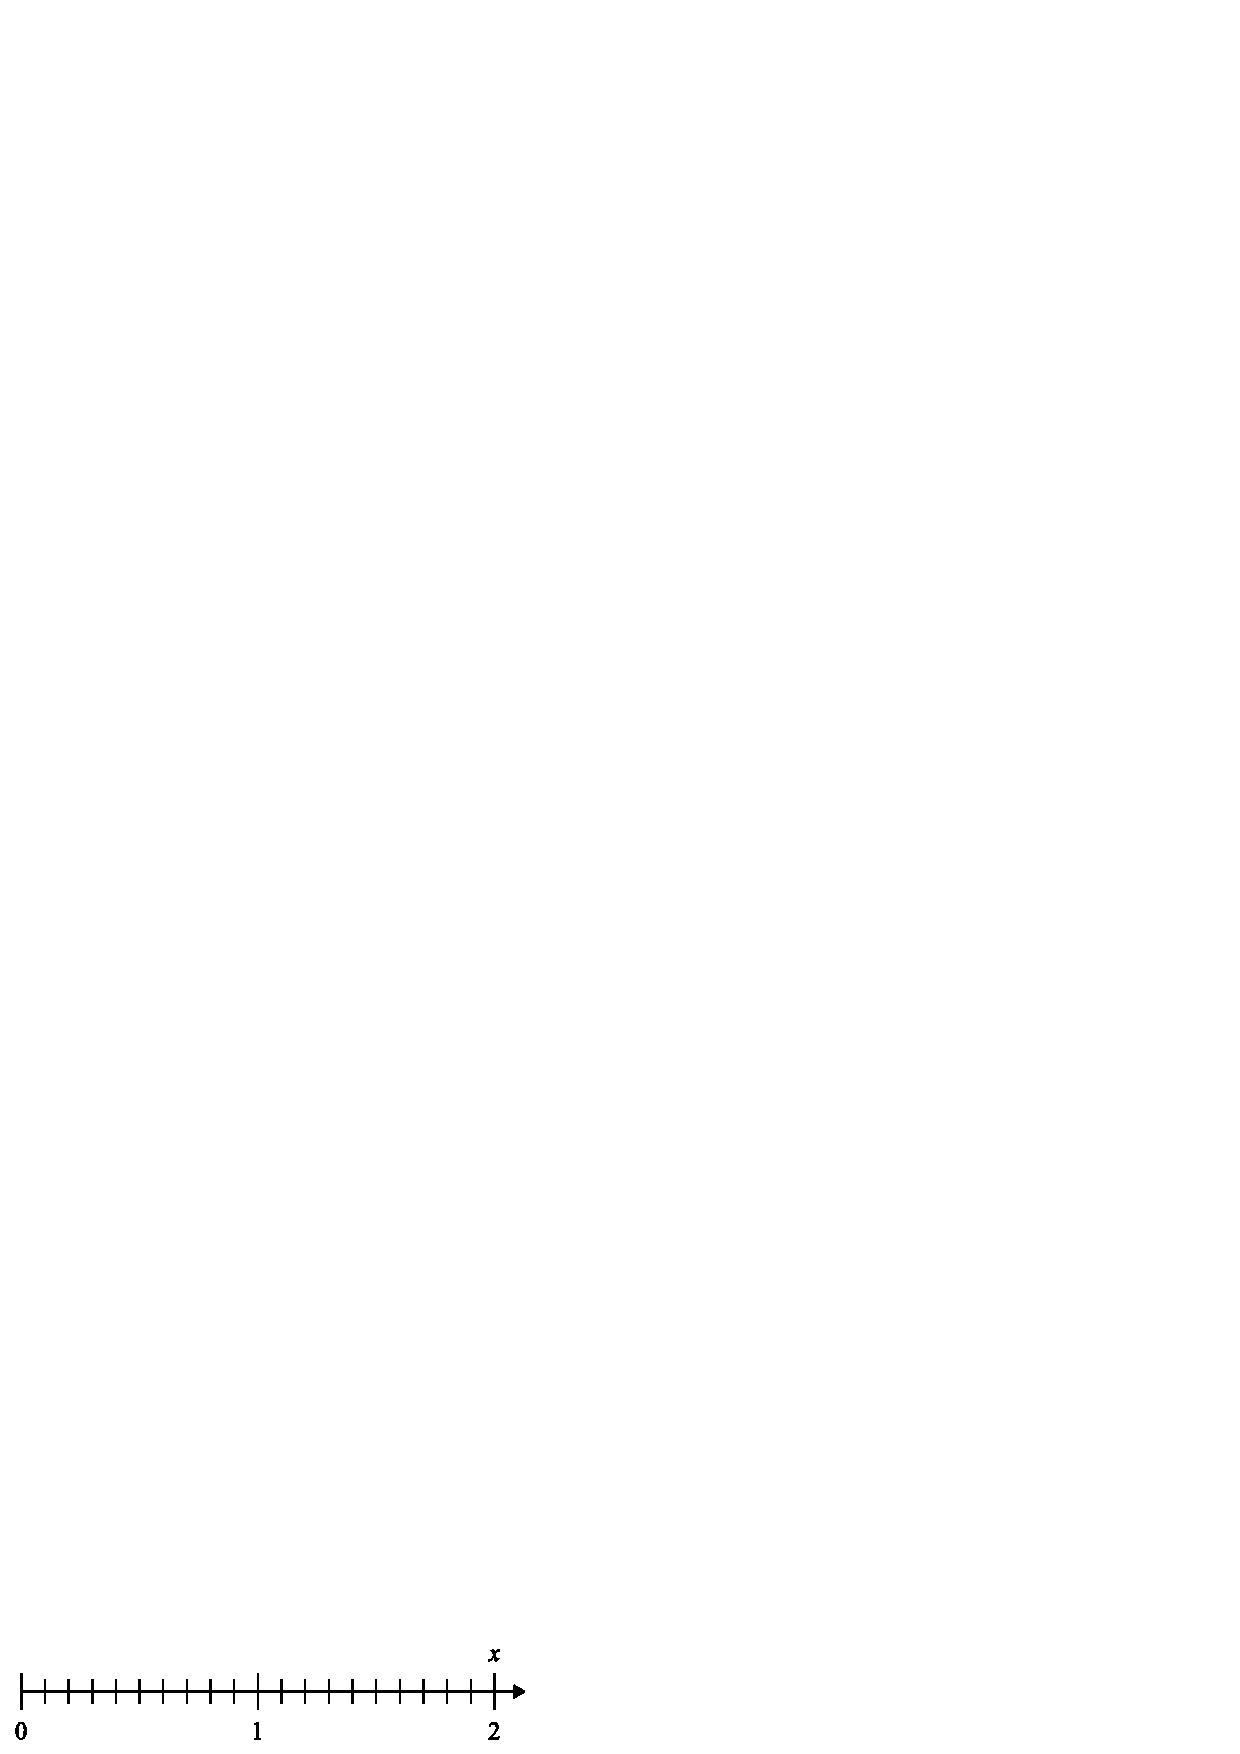
\includegraphics[width=7cm]{axe012x} \end{center}
\end{exercice}

%%%%%%%%%%%%%%%%%%%%%%%%%%%%%%%%%%%%%%%%%%%%%%%%%%%%%%%%%%%%%%%%%%%%%%%%%%%

\serie{Comparaison}

\begin{exercice}[Demi-droite graduée et comparaison]
\begin{enumerate}
 \item Reproduis la demi-droite graduée suivante et place les points $A(7,39)$ ; $B(7,46)$ et $C(7,425)$ :
\begin{center} 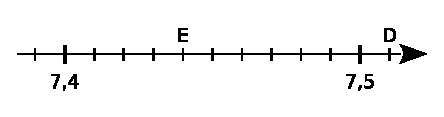
\includegraphics[width=6.6cm]{axe74E-75D} \end{center}
 \item Range dans l'ordre décroissant les abscisses de tous les points qui sont nommés.
 \end{enumerate}
\end{exercice}


\begin{exercice}[Rangement]
Range les nombres suivants dans l'ordre croissant :

5 ; 4,99 ; 4,9 ; 4,88 ; 5,000 1 ; 4,909 ; 4,879 :

\dotfill

\dotfill
\end{exercice}


\begin{exercice}[Rangement $(bis)$]
Range les nombres suivants dans l'ordre décroissant :

120 ; 119,999 ; 120,000 1 ; 120,101 ; 119,9 ; 119 ; 119,990 9 ; 120,100 1 ; 102,01 ; 120,1 :

\dotfill

\dotfill
\end{exercice}

%%%%%%%%%%%%%%%%%%%%%%%%%%%%%%%%%%%%%%%%%%%%%%%%%%%%%%%%%%%%%%%%%%%%%%%%%%%

\serie{Arrondir}

\begin{exercice}[Arrondir à l'unité]
Arrondis à l'unité les nombres suivants :
\begin{enumerate}
 \item 46,8 \dotfill ; 
 
 \item 109,75 \dotfill ; 
 
 \item 1,3 \dotfill ; 
 
 \item 0,09 \dotfill ; 
 
 \item 234,08 \dotfill ; 
 
 \item 4\,087,63 \dotfill. 
 
 \end{enumerate}
\end{exercice}

%%%%%%%%%%%%%%%%%%%%%%%%%%%%%%%%%%%%%%%%%%%%%%%%%%%%%%%%%%%%%%%%%%%%%%%%%%%

\serie{Encadrer}


\begin{exercice}[Encadrer à la dizaine]
235,5 ; 45 ; 1270 ; 574,23 ; 10\,095.
\end{exercice}


\begin{exercice}[Encadrer au dixième]
76,123 ; 461,99 ; 1\,254,01 ; 3,93 ; 9,99.
\end{exercice}


\begin{exercice}[Arrondir à la dizaine]
Arrondis à la dizaine les nombres suivants :
\begin{enumerate}
 \item 234,2 \dotfill ; 
 
 \item 3,14 \dotfill ; 
 
 \item 17,62 \dotfill ; 
 
 \item 889,3 \dotfill ; 
 
 \item 6\,289,3 \dotfill ; 
 
 \item 23,005 \dotfill. 
 
 \end{enumerate}
\end{exercice}


\begin{exercice}[Arrondir au dixième]
Arrondis au dixième les nombres suivants :
\begin{enumerate}
 \item 8,372 \dotfill ; 
 
 \item 50,64 \dotfill ; 
 
 \item 30,18 \dotfill ; 
 
 \item 43,725 \dotfill ; 
 
 \item 0,02 \dotfill ; 
 
 \item 78,66 \dotfill. 
 
 \end{enumerate}
\end{exercice}


\begin{exercice}
Dans chaque cas, propose, si cela est possible, un nombre entier que l'on peut intercaler entre les deux nombres donnés. 
Y a‑t‑il plusieurs solutions ? Si oui, cite‑les :
\begin{enumerate}
 \item $5 < …… < 6$ ;
 \item $6,4 < …… < 6,8$ ;
 \item $3,8 < …… < 5,3$ ;
 \item $6,5 < …… < 7,21$.
 \end{enumerate}
\end{exercice}


\begin{exercice}
Dans chaque cas, donne trois exemples différents de nombres décimaux que l'on peut intercaler entre les deux nombres donnés :
\begin{enumerate}
 \item $6 < …… < 7$ ;
 \item $4,5 < …… < 4,9$ ;
 \item $3,45 < …… < 3,48$ ;
 \item $6,8 < …… < 6,9$ ;
 \item $15,13 < …… < 15,14$ ;
 \item $3,238 < …… < 3,24$.
 \end{enumerate}
\end{exercice}


\begin{exercice}[Chiffres masqués]
Certains chiffres sont masqués par \#. Lorsque cela est possible, recopie et complète les pointillés avec $<$,$>$ ou $=$ :
\begin{enumerate} 
 \item $6,51 …… 6,7\#$ ;
 \item $5,42 …… 5,0\#$ ;
 \item $\#,23 …… 4,16$ ;
 \item $6,04 …… 6,1\#$ ;
 \item $3,\#35 …… 3,01$ ;
 \item $43,\#96 …… 43,0\#$.
 \end{enumerate}
\end{exercice}


\begin{exercice}[Nombres à trouver]
Dans chaque cas, recopie et complète les pointillés par un nombre décimal :
\begin{enumerate} 
 \item $24,5 < ...... < 24,6$ ;  
 
 \item $12,99 < ...... < 13$ ; 
 
 \item $32,53 < ...... < 32,54$ ; 
 
 \item $58 < ...... < 58,01$ ; 
 
 \item $5,879 < ...... < ...... < ...... < 5,88$. 

 \end{enumerate}
\end{exercice}

%%%%%%%%%%%%%%%%%%%%%%%%%%%%%%%%%%%%%%%%%%%%%%%%%%%%%%%%%%%%%%%%%%%%%%%%%%%

\serie{Techniques opératoires}


\begin{exercice}
Calcule mentalement les additions :
\begin{enumerate} 
 \item $4,6 + 5,2$ \dotfill ; 
 
 \item $6,2 + 3,4$ \dotfill ; 
 
 \item $4,5 + 6,1$ \dotfill ; 
 
 \item $8,3 + 9,6$ \dotfill ; 
 
 \item $8 + 1,5$ \dotfill ; 
 
 \item $8,6 + 8,9$ \dotfill ; 
 
 \item $3,9 + 5,4$ \dotfill ; 
 
 \item $6,5 + 8,7$ \dotfill ; 
 
 \item $6,8 + 9,4$ \dotfill ; 
 
 \item \hspace{0.1em} $12,9 + 15,8$ \dotfill. 

 \end{enumerate}
\end{exercice}


\begin{exercice}
Calcule mentalement les soustractions :
\begin{enumerate} 
 \item $6,5 - 4,3$ \dotfill ; 
 
 \item $7,6 - 0,4$ \dotfill ; 
 
 \item $4,9 - 4,3$ \dotfill ; 
 
 \item $5,7 - 0,4$ \dotfill ; 
 
 \item $4,7 - 4,3$ \dotfill ; 
 
 \item $6,2 - 4,6$ \dotfill ; 
 
 \item $9 - 8,7$ \dotfill ; 
 
 \item $3,1 - 1,8$ \dotfill ; 
 
 \item $7,8 - 6,9$ \dotfill ; 
 
 \item \hspace{0.2em}$17,4 - 8,7$ \dotfill. 
 
 \end{enumerate}  
\end{exercice}


\begin{exercice}
Calcule les sommes en effectuant des regroupements astucieux :
\begin{enumerate} 
 \item $6,5 + 12,6 + 1,5$ ;
 \item $36,99 + 45,74 + 2,01 + 13,26$ ;
 \item $9,25 + 8,7 + 5,3 + 16,75$ ;
 \item $34,645 + 34,75 + 2,25 + 4,355$ ;
 \item $7,42 + 4,2 + 7,8 + 25,58$ ;
 \item $3,01 + 2,9 + 6,1 + 7,99 + 2,001$.
 \end{enumerate}
\end{exercice}


\begin{exercice}
Pose et effectue :
\begin{enumerate} 
 \item $853,26 + 4 038,3$ ;
 \item $52 + 8,63 + 142,8$ ;
 \item $49,3 + 7,432 + 12,7$ ;
 \item $948,25 - 73,2$ ;
 \item $9,8 - 0,073$ ;
 \item $83 - 43,51$.
 \end{enumerate} 
 \end{exercice}


\begin{exercice}
Convertis en heures et minutes :\\
78 min ; 134 min ; 375 min ; 35 min ; 3\,840 s.
\end{exercice}


\begin{exercice}
Effectue les calculs :
\begin{enumerate} 
 \item 3 h 25 min $+$ 5 h 33 min ;
 \item 12 h 28 min $-$ 9 h 17 min ;
 \item 6 h 38 min $+$ 19 h 53 min ;
 \item 21 h 15 min $-$ 9 h 29 min ;
 \item 5 h 13 min 33 s $+$ 9 h 45 min 47 s ;
 \item 9 h 6 min 15 s $-$ 8 h 39 min 36 s.
 \end{enumerate}
\end{exercice}


\begin{exercice}
Calcule mentalement :
\begin{enumerate} 
 \item $4,357 \cdot 100$ \dotfill ; 
 
 \item $89,7 \cdot 1\,000$ \dotfill ; 
 
 \item $0,043 \cdot 10$ \dotfill ; 
 
 \item $0,28 \cdot 1\,000$ \dotfill ; 
 
 \item $39 \cdot 100$ \dotfill ; 
 
 \item $0,48 \cdot 10$ \dotfill ; 
 	
 \item $354 \cdot 10$ \dotfill ; 
 	
 \item $0,03 \cdot 10\,000$ \dotfill ; 
 
 \end{enumerate}
\end{exercice}


\begin{exercice}
Calcule mentalement :
\begin{enumerate} 
 \item $4\,338 : 10$ \dotfill ; 
 
 \item $1\,297 : 1\,000$ \dotfill ; 
 	
 \item $12,3 : 10$ \dotfill ; 
 
 \item $0,87 : 100$ \dotfill ; 
 	
 \item $3,8 : 1\,000$ \dotfill ; 
 
 \item $0,04 : 100$ \dotfill ; 
 	
 \item $354 : 10$ \dotfill ; 
 
 \item $12,5 : 100$ \dotfill. 
 
 \end{enumerate}
\end{exercice}


\begin{exercice}
Calcule mentalement :
\begin{enumerate} 
 \item $435,7 \cdot 0,1$ \dotfill ; 
 
 \item $18,73 \cdot 0,01$ \dotfill ; 
 
 \item $439,345 \cdot 0,001$ \dotfill ; 
 
 \item $0,28 \cdot 0,1$ \dotfill ; 
 
 \item $39 \cdot 0,001$ \dotfill ; 
 
 \item $0,8 \cdot 0,01$ \dotfill ; 
 
 \item $354 \cdot 0,001$ \dotfill ; 
 
 \item $0,03 \cdot 0,001$ \dotfill. 
 
 \end{enumerate}
\end{exercice}

\begin{exercice}
Calcule mentalement :
\begin{enumerate} 
 \item $48 \div 0,1$ \dotfill ; 
 
 \item $12,97 \div 0,01$ \dotfill ; 

 \item $12,3 \div 0,001$ \dotfill ; 
 
 \item $0,45 \div 0,1$ \dotfill ; 
 	
 \item $5,61 \div 0,0001$ \dotfill ; 
 	
 \item $0,056 \div 0,1$ \dotfill ; 
 
 \item $354 \div 0,001$ \dotfill ; 
 
 \item $0,5 \div 0,001$ \dotfill. 

 \end{enumerate}
\end{exercice}


\begin{exercice}
Complète par 10 ; 100 ; 1\,000 ; 10\,000 \ldots :
\begin{enumerate} 
 \item $8,79 \cdot \dotfill = 87,9$ ; 
 
 \item $4,35 \cdot \dotfill = 43\,500$ ; 
 
 \item $0,837 \cdot \dotfill = 8,37$ ; 
 
 \item $0,367 \cdot \dotfill = 3,67$ ; 
 
 \item $0,028 \cdot \dotfill = 0,28$ ; 
 
 \item $0,17 \div \dotfill = 0,017$ ; 
 
 \item $23 \div \dotfill = 0,23$ ; 
 
 \item $480 \div \dotfill = 4,8$ ; 
 
 \item $900 \div \dotfill = 0,09$ ; 
 
 \item \hspace{0.25em}$18\,000 \div \dotfill = 18$. 
 
 \end{enumerate}
\end{exercice}


\begin{exercice}
Complète par le signe opératoire qui convient :
\begin{colenumerate}{2}
 \item $0,8 \ldots 100 = 80$ ;
 \item $0,38 \ldots 10 = 0,038$ ;
 \item $47 \ldots 100 = 0,47$ ;
 \item $380 \ldots 10 = 38$ ;
 \item $5 \ldots 0,1 = 0,5$ ;
 \item $60\,000 \ldots 10 = 6\,000$ ;
 \item $4\,100 \ldots 100 = 4\,000$ ;
 \item $5\,600 \ldots 100 = 56$ ;
 \item $8 \ldots 0,01 = 0,08$ ;
 \item \hspace{0.25em}$100 \ldots 1,2 = 120$.
 \end{colenumerate} 
\end{exercice}


\begin{exercice}
Calcule mentalement en détaillant ta démarche :
\begin{enumerate} 
 \item $0,1 \cdot 14 \cdot 1\,000$ \dotfill ; 
 
 \item $2,18 \cdot 0,001 \cdot 100$ \dotfill ; 

 \item $1,8 \cdot 0,01 \cdot 10$ \dotfill ; 

 \item $4 •\cdot 0,01 \cdot 100$ \dotfill. 

 \end{enumerate} 
\end{exercice}


\begin{exercice}
Sachant que $48 \cdot 152 = 7\,296$, détermine les résultats des calculs :
\begin{enumerate} 
 \item $48 \cdot 1,52$ \dotfill ; 
 
 \item $4,8 \cdot 15,2$ \dotfill ; 
 
 \item $0,48 \cdot 0,152$ \dotfill ; 
 
 \item $0,048 \cdot 1\,520$ \dotfill. 

 \end{enumerate} 
\end{exercice}


\begin{exercice}
Calcule en regroupant astucieusement :
\begin{enumerate} 
 \item $0,8 \cdot 2 \cdot 0,6 \cdot 50$ \dotfill ; 
 
 \item $0,25 \cdot 12,38 \cdot 4$ \dotfill ; 
 
 \item $8 \cdot 49 \cdot 1,25$ \dotfill ; 
 
 \item $2,5 \cdot 12,9 \cdot 0,04$ \dotfill ; 
 
 \item $0,15 \cdot 70 \cdot 0,02$ \dotfill ; 
 
 \item $75 \cdot 0,06 \cdot 0,4$ \dotfill. 
 
 \end{enumerate} 
\end{exercice}


\begin{exercice}
Place correctement la virgule dans le résultat de la multiplication (en ajoutant éventuellement un ou des zéros) :
\begin{enumerate} 
 \item $12,8 \cdot  5,3 = \textcolor{PartieGeometrie}{6\,784}$ ;
 \item $28,7 \cdot 1,04 = \textcolor{PartieGeometrie}{29\,848}$ ;
 \item $0,15 \cdot 6,3 = \textcolor{PartieGeometrie}{945}$ ;
 \item $0,008 \cdot 543,9 = \textcolor{PartieGeometrie}{43\,512}$ ;
 \item $0,235 \cdot 0,132 = \textcolor{PartieGeometrie}{3\,102}$.
 \end{enumerate}
\end{exercice}


\begin{exercice}
Place la virgule dans le nombre écrit en \textcolor{BleuOuv}{bleu} pour que l'égalité soit vraie :
\begin{enumerate} 
 \item $3,42 \cdot \textcolor{BleuOuv}{271} = 9,268\,2$ ;
 \item $\textcolor{BleuOuv}{432} \cdot 0,614 = 26,524\,8$ ;
 \item $0,48 \cdot \textcolor{BleuOuv}{62} = 29,76$ ;
 \item $2,6 \cdot \textcolor{BleuOuv}{485} = 126,1$ ;
 \item $\textcolor{BleuOuv}{45} \cdot 29,232 = 131,544$.
 \end{enumerate}
\end{exercice}

\begin{exercice}
Pose et effectue les produits :
\begin{enumerate} 
 \item $2,08 \cdot 4,23$ \dotfill ; 
 
 \item $4,38 \cdot 5,7$ \dotfill ; 
 
 \item $6,93 \cdot 15,8$ \dotfill ; 
 
 \item $8,35 \cdot 0,18 $\dotfill.  
 \end{enumerate}
\end{exercice}


\begin{exercice} 
Calcule mentalement :
\begin{colenumerate}{2}
 \item $ 8,6 \div 2$ ;
 \item $ 24,8 \div 4$ ;
 \item $ 8,8 \div 8$ ;
 \item $ 7,7 \div 11$ ;
 \item $ 15,6 \div 3$ ;
 \item $ 63,6 \div 6$.
 \end{colenumerate}
\end{exercice}


\begin{exercice} 
Pose et effectue les divisions suivantes pour en trouver le quotient décimal exact :
\begin{enumerate} 
 \item $ 12,6 \div 6$ \dotfill ; 
 
 \item $ 28,48 \div 4$ \dotfill ; 

 \item $ 169,2 \div 3$ \dotfill ; 

 \item $ 0,162 \div 9$ \dotfill ; 

 \item $ 67,5 \div 4$ \dotfill ; 

 \item $ 9,765 \div 15$ \dotfill. 
 \end{enumerate}
\end{exercice}


\begin{exercice}[Valeurs approchées] 
\begin{enumerate} 
 \item Pose et effectue les divisions suivantes jusqu'au millième :
 \begin{itemize}
  \item $12 \div 7$ \dotfill ; 
  
  \item $148,9 \div 12$ \dotfill ; 
  
  \item $13,53 \div 3$ \dotfill. 
  \end{itemize}
 \item Pose et effectue les divisions suivantes jusqu'au centième :
  \begin{itemize}
  \item $123,8 \div 7$ \dotfill ; 
  
  \item $235,19 \div 11$ \dotfill ; 
  
  \item $0,14 \div 3$ \dotfill. 
  \end{itemize}
 \end{enumerate}
\end{exercice}


\begin{exercice} 
Calcule la valeur exacte ou une valeur arrondie au centième des divisions suivantes :
\begin{enumerate} 
 \item $1 \div 2,74$ \dotfill ; 

 \item $5,87 \div 2,3$ \dotfill ; 

 \item $3,24 \div 1,7$ \dotfill ; 

 \item $45,6 \div 0,24$ \dotfill ; 

 \item $20,35 \div 8,5$ \dotfill ; 

 \item $0,53 \div 0,17$ \dotfill. 
 \end{enumerate}
\end{exercice}


\begin{exercice} 
Calcule la valeur exacte ou une valeur arrondie au centième des divisions suivantes :
\begin{enumerate} 
 \item $3,35 \div 0,42$ \dotfill ; 

 \item $41,5 \div 3,14$ \dotfill ; 

 \item $ 0,03 \div 2,1$ \dotfill ; 

 \item $0,35 \div 0,25$ \dotfill ; 

 \item $0,53 \div 0,8$ \dotfill ; 

 \item $21,7 \div 0,14$ \dotfill. 
 \end{enumerate}
\end{exercice}

%%%%%%%%%%%%%%%%%%%%%%%%%%%%%%%%%%%%%%%%%%%%%%%%%%%%%%%%%%%%%%%%%%%%%%%%%%%

\serie{Heures, minutes, secondes}


\begin{exercice}
Pose et effectue les opérations suivantes :
\begin{enumerate} 
 \item 18 h 15 min 22 s $+$ 9 h 37 min 43 s ;
 \item 12 h 26 min 52 s $-$ 7 h 39 min 57 s ;
 \item 9 h 38 min 22 s $+$ 4 h 59 min 34 s ;
 \item 12 h 40 min 21 s $-$ 6 h 35 s.
 \end{enumerate}
\end{exercice}


\begin{exercice}
Pose et effectue les opérations suivantes :
\begin{enumerate} 
 \item 13 h 25 min 42 s $+$ 12 h 35 min 52 s ;
 \item 15 h 43 min 08 s $-$ 6 h 51 min 34 s ;
 \item 10 h 41 s $+$ 9 h 57 min 49 s ;
 \item 21 h $-$ 17 h 31 min 32 s.
 \end{enumerate}
\end{exercice}


\begin{exercice}
Un randonneur part en promenade à 9 h 30. Il rentre à 12 h 05, ne s'étant arrêté pour se reposer que lors de trois pauses de 5 min chacune. Pendant combien de temps ce randonneur a‑t‑il marché ?
\end{exercice}


\begin{exercice}
Pierre part de chez lui à 9 h 55 pour aller faire des courses. Il met 12 min pour se rendre au supermarché et il y reste pendant 1 h 35 min.
\begin{enumerate} 
 \item À quelle heure repart‑il du supermarché ?
 \item Il rentre ensuite chez lui et y arrive à 12 h 01. Combien de temps son trajet de retour a‑t‑il duré ?
 \end{enumerate}
\end{exercice}


\begin{exercice}
Sarah a noté les heures de lever et de coucher du Soleil en septembre 2008. Le $1^{er}$ septembre, le Soleil s'est levé à 7 h 09 et il s'est couché à 20 h 31. Le 30 septembre, le Soleil s'est levé à 7 h 50 et il s'est couché à 19 h 30. De quelle durée les jours ont‑ils diminué au mois de septembre 2008 ?
\end{exercice}
 